\documentclass[preprint,12pt,authoryear]{elsarticle}

\usepackage[margin=2.4cm]{geometry}
\usepackage{fontspec}
\setmainfont{Times New Roman}
\setmonofont{Menlo}[Scale=0.86]
\usepackage{amsmath,amssymb,amsfonts}
\usepackage{algorithm}
\usepackage{algorithmic}
\usepackage{booktabs}
\usepackage{graphicx}
\usepackage{multirow}
\usepackage{lineno}
\usepackage{url}
\usepackage{xcolor}

\journal{Computers and Electronics in Agriculture}

\newcommand{\BA}{\mathrm{BA}}
\setlength{\emergencystretch}{1.8em}

\begin{document}

\begin{frontmatter}

\title{Budget-Amortized Source-Anchored Adaptation for Bandwidth-Limited Orchard Cameras: Paid Supervision, Streaming Deferral, and Quantization Audit}

\author[1]{Weicheng Tong\corref{cor1}}
\ead{Sver0411@outlook.com}
\cortext[cor1]{Corresponding author.}

\affiliation[1]{organization={Shandong Agriculture and Engineering University},
            city={Jinan},
            state={Shandong},
            country={China}}

\begin{abstract}
Low-power camera nodes deployed for foliar disease screening in commercial orchards routinely face two coupled bottlenecks: severe cross-orchard domain shift and tight wireless uplink quotas. Under a fixed communication allowance, a field camera must trade off two competing expenditures of uplink bytes: uploading a small batch of orchard photographs for remote agronomic annotation so a new local classifier head can be fitted, or keeping its factory model frozen and forwarding uncertain frames to a cloud vision model. Existing cascade and learning-to-defer evaluations usually treat calibration labels as free, rank frames offline over a full test batch, or run exclusively in 32-bit floating point (FP32) without accounting for microcontroller INT8 quantization. Here we formulate paid remote supervision and strictly causal single-frame streaming deferral on a single unified byte ledger under both upfront (\emph{prepaid}) and zero-initial-credit (\emph{earned}) funding schedules, and introduce \emph{Budget-Amortized Source-Anchored Adaptation (BASA)}. BASA couples horizon-amortized label budgeting, label-free quantile-stratified candidate selection, convex \emph{Anisotropic Source-Anchored Regularization (ASAR)} packed into a 1,294-byte \texttt{EQ01} INT8 classifier head, and a causal 64-frame rolling-percentile deferral gate with an optional one-sided recall guard. Across three decontaminated apple-leaf cohorts (Cornell, Kashmir, and date-split Latvia), three edge pipelines (MobileNetV2 FP32, ESP32-S3 host quantization replay, and MobileNetV4-Conv-Small), 13 fixed-cap baselines, and three budget-clamped baselines, BASA obtains the highest mean balanced accuracy across all 36 primary 25\%-uplink settings (73.50\% overall; 74.49\% prepaid; 72.52\% earned), outperforming fixed-cap baselines by +1.46 to +5.35 percentage points (pp) and budget-clamped baselines by +0.58 to +0.89~pp overall (+1.14 to +1.36~pp under earned credit). BASA also leads at a 10\% scarce uplink (70.49\% vs.\ 69.40\% for budget-clamped cross-entropy), while revealing an honest operating boundary at a generous 50\% uplink where budget-clamped cross-entropy slightly edges ahead (75.56\% vs.\ 75.29\%). We further document that ESP32-S3 INT8 quantization reverses up to 13/45 pairwise router rankings, and validate the standalone C99 runtime directly on an ESP32-S3 N16R8 microcontroller (160~MHz): 93~$\mu$s head inference, 41~$\mu$s gating (0.025\% of backbone latency), 1,836~B persistent state, and zero bit-level mismatches.
\end{abstract}

\begin{highlights}
\item Unified byte ledger couples paid orchard labels with causal streaming deferral.
\item BASA beats 13 fixed-cap and 3 budget-clamped baselines at 10\% and 25\% uplinks.
\item Anisotropic source anchoring prevents MobileNetV4 collapse on shifted orchards.
\item ESP32-S3 INT8 quantization reverses up to 13/45 pairwise router rankings.
\item On-chip ESP32-S3 execution takes 134~$\mu$s per frame using 1,836~B persistent RAM.
\end{highlights}

\begin{keyword}
Precision agriculture \sep Orchard disease screening \sep Edge intelligence \sep Learning to defer \sep Microcontroller quantization \sep ESP32-S3
\end{keyword}

\end{frontmatter}

\linenumbers

\section{Introduction}
\label{sec:intro}

Battery-powered visual sensors are increasingly used to flag foliar diseases early in commercial orchards, reducing scouting labor and delaying chemical intervention until lesions appear \citep{mohanty2016,agri}. Running a compact convolutional neural network directly on a microcontroller unit (MCU) such as an ESP32-S3 allows continuous local screening without streaming raw video over rural cellular or low-power wide-area links. The catch is well documented in agricultural computer vision: classifiers trained on laboratory or web-scraped leaf images lose substantial accuracy once moved to an unseen orchard with different illumination, soil and canopy backgrounds, cultivars, and disease prevalence \citep{mohanty2016,singh2020}.

When an intermittent wireless uplink is available, a field camera has two practical ways to spend its byte allowance:
\begin{enumerate}
  \item \textbf{Selective remote review (deferral):} keep the factory edge model frozen and transmit compressed JPEG frames that look uncertain to a stronger cloud vision model \citep{jitkrittum2023,edgeboost}.
  \item \textbf{Supervised local adaptation:} transmit a small set of target-orchard photographs and quantized penultimate activations so an agronomist or cloud service can label them, fit a lightweight updated classifier head, and return it over the air \citep{tinyol,lin2022}.
\end{enumerate}

On a real rural link, these two choices draw from the same communication budget. Downloading a linear classification head takes only 1,294 bytes, yet the remote annotator still has to inspect the actual calibration photographs to assign ground-truth labels. Buying too many target labels leaves too few bytes for deferring hard frames later in the monitoring window. The penalty is sharper still when the camera starts with \emph{zero initial credit} (an \emph{earned} byte schedule that accrues allowance frame by frame without borrowing): saving up for a large calibration batch delays head installation across a sizeable share of the deployment window, forcing the camera to serve unadapted factory predictions in the meantime. Conversely, buying only 16--32 labels and refitting an unconstrained 1,280-dimensional linear head from scratch easily overfits modern pretrained backbones such as MobileNetV4 \citep{mobilenetv4}, collapsing recall on shifted sites.

Most work on model cascades and learning to defer \citep{ova,compareconf,jitkrittum2023,edgeboost,mao2025,gatekeeper} focuses on optimizing the deferral score assuming training labels are already in hand, and often evaluates routers offline by sorting an entire test batch. Continuous video-analytics schedulers such as Ekya \citep{ekya} and Remembrall \citep{remembrall} jointly allocate retraining and inference resources, but target GPU-class edge servers rather than kilobyte-constrained MCUs. Just as importantly, deferral benchmarks are almost always executed in 32-bit floating point (FP32), leaving open whether INT8 quantization on an embedded processor changes which router actually performs best.

Anchored to the open-source AgriTinyVision ESP32-S3 release \citep{agri}, this study evaluates paid remote supervision and strictly causal single-frame deferral on a single byte-exact ledger and proposes \emph{Budget-Amortized Source-Anchored Adaptation (BASA)}. Our main findings and contributions are as follows:
\begin{enumerate}
  \item \textbf{Unified single-ledger formulation:} We account for calibration JPEGs, quantized activation packets, model-return wire bytes, and online inference JPEGs on one ledger under both upfront (\emph{prepaid}) and zero-initial-credit (\emph{earned}) funding schedules, characterizing the double opportunity cost incurred by calibration overhead under earned credit.
  \item \textbf{BASA controller:} We combine horizon-amortized label budgeting, label-free quantile-stratified selection, and \emph{Anisotropic Source-Anchored Regularization (ASAR)}---a convex orthogonal shrinkage family around the factory classifier direction $\hat{\mathbf{w}}_0$ selected via temperature-invariant out-of-fold discrimination and packed into the 1,294-byte \texttt{EQ01} INT8 format.
  \item \textbf{Multi-site, multi-backbone, and budget-clamped evaluation:} Across three decontaminated apple-leaf datasets (Cornell, Kashmir, and chronologically split Latvia), three edge pipelines (MobileNetV2 FP32, ESP32-S3 host INT8 replay, and MobileNetV4-Conv-Small), 13 fixed-cap baselines, and three stronger budget-clamped baselines, BASA achieves the highest mean balanced accuracy at both 10\% (70.49\%) and 25\% (73.50\%) uplink rates while documenting the 50\% abundant-uplink crossover where budget-clamped cross-entropy edges ahead (75.56\% vs.\ 75.29\%).
  \item \textbf{Quantization audit, recall guard, and ESP32-S3 silicon validation:} We show that serving FP32-fitted heads on ESP32-S3 quantized activations reverses up to 13/45 pairwise router rankings, evaluate a one-sided recall guard that cuts Latvian apple-scab misses by more than half on MobileNetV2, and measure the standalone C99 runtime directly on an ESP32-S3 N16R8 board (134~$\mu$s combined per-frame overhead, 1,836~B persistent state, 0/16 bit-level mismatches).
\end{enumerate}

\section{Related Work}
\label{sec:related}

\subsection{Field Shift in Agricultural Edge Vision}
Early leaf-disease benchmarks such as PlantVillage reported near-perfect in-domain accuracy that fell sharply on unconstrained field photographs \citep{mohanty2016}. Subsequent datasets---including PlantDoc \citep{singh2020}, the Cornell FGVC7 apple-pathology set \citep{cornell}, an indigenous Kashmir apple-leaf collection \citep{kashmir}, and the AppleScabLDs Latvian orchard archive \citep{latvia}---exposed substantial variation in background foliage, camera sensors, and label granularity (general foliar abnormality versus single-pathogen apple scab). The AgriTinyVision project \citep{agri} deployed a quantized 160-pixel MobileNetV2 on an ESP32-S3 N16R8 microcontroller and archived paired board/FP32 field-validation logs, providing the physical hardware baseline for this work.

\subsection{Model Cascades and Learning to Defer}
Selective offloading routes uncertain local inferences to a remote expert. \citet{edgeboost} filter edge predictions using a temperature-calibrated top-two probability margin (EdgeBoost). Learning-to-defer methods jointly model local and expert errors through one-vs-all surrogates \citep{ova}, exact confidence comparison \citep{compareconf}, difference-of-probabilities regression \citep{jitkrittum2023}, two-stage cost-sensitive surrogates \citep{mao2025}, and confidence-tuned cascades \citep{gatekeeper}. Unlike those benchmarks, we bill the exact byte cost of purchasing target-site calibration labels and downloading router parameters onto the same ledger as inference JPEGs, restrict every router to causal single-frame decisions, and check whether method rankings survive MCU INT8 quantization.

\subsection{On-Device Adaptation and Bandwidth-Aware Scheduling}
Updating only the final linear layer on microcontrollers is well established in TinyML \citep{tinyol,lin2022}. On GPU-equipped edge servers, \citet{ekya} and \citet{remembrall} schedule continuous retraining alongside live video inference, while black-box shift detectors such as BBSD-soft \citep{bbsd} monitor unlabelled prediction distributions to trigger intervention. Our work examines the distinct kilobyte-budgeted MCU regime: deciding how many target labels a camera can afford relative to its deployment horizon and funding schedule, and regularizing small-sample head updates around the factory classifier so pretrained representations are not degraded.

\section{Materials and Methods}
\label{sec:methods}

\subsection{System Model and Unified Single-Ledger Byte Contract}
\label{sec:model}

Consider an orchard camera operating over a scheduled monitoring window of $N$ image arrivals indexed by $t \in \{0, 1, \dots, N-1\}$ (Fig.~\ref{fig:arch}). At each arrival, the node captures an RGB photograph, runs its frozen visual backbone to obtain a $d$-dimensional penultimate activation $\mathbf{x}_t \in \mathbb{R}^d$ ($d = 1{,}280$ for both MobileNetV2 and MobileNetV4-Conv-Small) and factory source probability $p_0(\mathbf{x}_t) \in [0,1]$, and encodes a single quality-75 JPEG (224-pixel maximum long edge) of measured size $s_t$ bytes. Memory is limited to one evaluation frame at a time; future scores, labels, and JPEG lengths are never visible.

\begin{figure}[t]
  \centering
  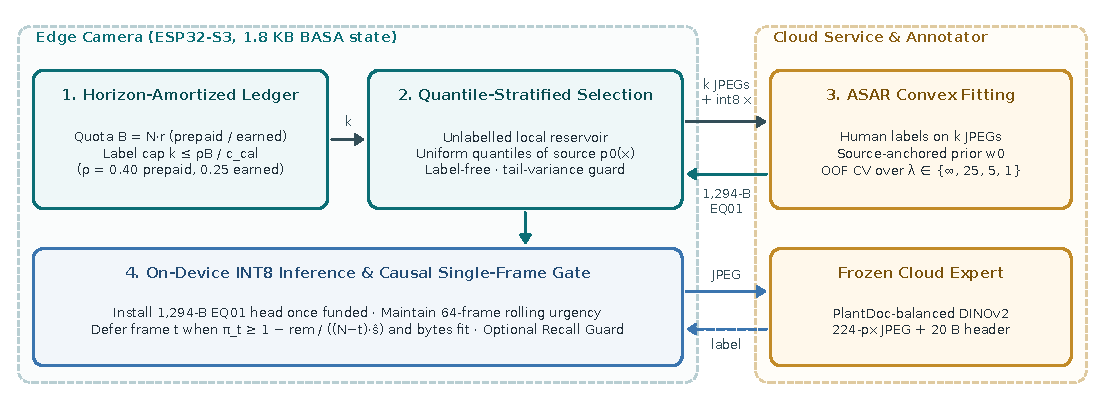
\includegraphics[width=\textwidth]{figures/compag_basa_arch.pdf}
  \caption{System architecture of Budget-Amortized Source-Anchored Adaptation (BASA). Paid remote annotation, 1,294-byte \texttt{EQ01} INT8 head installation, and causal single-frame JPEG deferral debit one unified byte ledger under either prepaid or zero-initial-credit (earned) funding.}
  \label{fig:arch}
\end{figure}

Let $r$ denote the nominal uplink allowance in application bytes per arrival, yielding window quota $B = Nr$. Anchored to empirical full-review traffic on Cornell ($\approx 6{,}800$~B/frame), we set the primary contract to 25\% ($r = 1{,}700$~B/frame) and sweep 10\% ($r = 680$~B/frame) and 50\% ($r = 3{,}400$~B/frame). Every calibration, control, and review packet debits the same ledger:
\begin{itemize}
  \item \textbf{Remote calibration label:} one quality-75 JPEG ($s_i$), an 8-byte envelope, a 1,293-byte symmetric signed-INT8 activation record (4-byte ID, 1-byte label, 4-byte float32 scale, and $d=1{,}280$ signed bytes), a 4-byte source score, and a 12-byte receipt, totaling $c_{\mathrm{cal}}(i) = s_i + d + 37$ bytes.
  \item \textbf{Head transaction and wire return:} a 32-byte setup request, an 8-byte action header, and a packed \texttt{EQ01} INT8 classifier head of $c_{\mathrm{head}} = d + 14 = 1{,}294$ bytes (4-byte magic, 2-byte dimension, 4-byte float32 scale, 4-byte float32 bias, and $d$ weights in $[-127, 127]$), giving fixed overhead $c_0 = 1{,}334$ bytes. Learned deferral baselines additionally pay their exact serialized router weights (e.g., an extra 1,294~B for two-head routers such as OvA, CompareConfidence, and Mao two-stage).
  \item \textbf{Online inference review:} the current 224-pixel JPEG plus 20 application header bytes, $c_{\mathrm{rev}}(t) = s_t + 20$, forwarded to a frozen cloud expert (PlantDoc-balanced DINOv2-small; \citealp{dino}).
\end{itemize}

We evaluate two funding schedules sharing the same total quota $B$:
\begin{equation}
  F_t =
  \begin{cases}
    B, & \text{Prepaid (upfront grant)}, \\
    (t + 1) r, & \text{Earned (zero initial credit)}.
  \end{cases}
  \label{eq:funding}
\end{equation}
Any causal controller spending $u_t$ bytes at step $t$ must obey the prefix no-overdraft constraint
\begin{equation}
  \sum_{\tau=0}^{t} u_\tau \le F_t, \qquad \forall t \in \{0, \dots, N-1\}.
  \label{eq:overdraft}
\end{equation}
Let $S(k) = c_0 + \sum_{i \in \mathcal{I}_k} c_{\mathrm{cal}}(i)$ be the total setup cost of purchasing $k$ target labels from an unlabelled local reservoir $\mathcal{R}$, and define the supervision share $\rho = S(k)/B$. Under prepaid funding, the updated head takes effect at $t = 0$ and leaves $(1-\rho)B$ bytes for online deferral. Under earned funding, the camera must serve unadapted factory predictions while accumulating bytes until $t_{\mathrm{act}} = \lceil S(k)/r \rceil - 1 \approx \rho N$. Setup expenditure under earned credit therefore carries a double opportunity cost: it shrinks the remaining online review budget by $\rho$ and leaves the first $\rho N$ arrivals both unadapted and unqueried.

Because disease prevalence varies widely across orchards (66.7\%--87.6\%), raw accuracy can mask trivial all-positive behavior. Our primary metric is balanced accuracy,
\begin{equation}
  \BA = \frac{1}{2}\left(\frac{\mathrm{TP}}{\mathrm{TP}+\mathrm{FN}} + \frac{\mathrm{TN}}{\mathrm{TN}+\mathrm{FP}}\right),
  \label{eq:ba}
\end{equation}
accompanied by raw false-positive ($\mathrm{FP}$) and false-negative ($\mathrm{FN}$) counts on the scab-triage cohort where missed lesions dominate operational risk.

\subsection{Budget-Amortized Source-Anchored Adaptation (BASA)}
\label{sec:basa}

BASA coordinates supervision sizing, sample selection, regularized fitting, and online deferral in four leak-free stages (Algorithm~\ref{alg:basa}).

\subsubsection{Horizon-Amortized Supervision Budgeting}
Before buying any label, the node computes the mean per-label byte cost $\bar{c}_{\mathrm{cal}}$ over the unlabelled local reservoir $\mathcal{R}$ (up to the authorized cap $L_{\max} \in \{32, 128\}$). Accounting for the double opportunity cost of earned credit, BASA caps planned setup expenditure at $\rho_{\mathrm{pre}} = 0.40$ under prepaid funding and $\rho_{\mathrm{earn}} = 0.25$ under earned funding:
\begin{equation}
  k = \min\!\left(L_{\max},\; k_{\mathrm{half}},\; \max\!\left(k_{\min},\; \left\lfloor \frac{\rho B - c_0}{\bar{c}_{\mathrm{cal}}} \right\rfloor\right)\right),
  \label{eq:amort}
\end{equation}
where $k_{\min} = 16$ and $k_{\mathrm{half}} = \lfloor (0.5B - c_0)/\bar{c}_{\mathrm{cal}} \rfloor$ ensures that at least half of $B$ remains available for online deferral (falling back to frozen review if $k_{\mathrm{half}} < 8$). On short horizons such as Kashmir ($N = 384$), this rule automatically scales setup down to $k \approx 16$ under earned credit rather than starving deferral, whereas on longer horizons such as Cornell ($N = 1{,}353$) it amortizes larger batches ($k = 32$ or $k \approx 70$).

\subsubsection{Label-Free Quantile-Stratified Acquisition}
Under skewed orchard prevalence, taking the first $k$ unlabelled arrivals at random often yields severe class imbalance (fewer than two negatives in roughly 10\% of 16-image draws). BASA sorts $\mathcal{R}$ by the camera's own factory probability $p_0(\mathbf{x})$, splits the sorted list into $k$ contiguous quantile bins, and picks the median-ranked item from each bin. No labels are touched prior to purchase, yet the purchased panel spans low-score negatives, uncertain boundary cases, and high-score positives.

\subsubsection{Anisotropic Source-Anchored Regularization (ASAR)}
Given $k$ purchased pairs $\{(\mathbf{q}_i, y_i)\}_{i=1}^k$, let $\tilde{\mathbf{x}}_i = \mathbf{q}_i / \|\mathbf{q}_i\|_2$ be L2-normalized INT8 activations with inverse-frequency class weights $\omega_i = k / (2 n_{y_i})$. Standard isotropic $L_2$ logistic regression shrinks $\mathbf{w}$ toward $\mathbf{0}$, throwing away the pretrained source classifier direction $\hat{\mathbf{w}}_0 = \mathbf{w}_0 / \|\mathbf{w}_0\|_2$ (extracted from the released ONNX or \texttt{source.bin} head).

Decomposing $\mathbf{w}$ orthogonally into $\Pi_0 \mathbf{w} + \Pi_\perp \mathbf{w}$, where $\Pi_0 = \hat{\mathbf{w}}_0 \hat{\mathbf{w}}_0^\top$ and $\Pi_\perp = I - \Pi_0$, ASAR solves the strictly convex problem
\begin{equation}
  \min_{\mathbf{w} \in \mathbb{R}^d,\, b \in \mathbb{R}} \;
  \sum_{i=1}^{k} \omega_i \log\!\left(1 + e^{-(2y_i-1)(\mathbf{w}^\top \tilde{\mathbf{x}}_i + b)}\right)
  + \frac{1}{2}\|\Pi_0 \mathbf{w}\|_2^2 + \frac{\lambda}{2}\|\Pi_\perp \mathbf{w}\|_2^2.
  \label{eq:asar}
\end{equation}
At $\lambda = 1$, $\Pi_0 + \Pi_\perp = I$ recovers standard isotropic $L_2$ logistic regression ($C=1$). At $\lambda \to \infty$, $\Pi_\perp \mathbf{w} = \mathbf{0}$ yields two-parameter Platt recalibration ($a\,\hat{\mathbf{w}}_0^\top \tilde{\mathbf{x}} + b$, $a \ge 0$) along the factory direction. For finite $\lambda > 1$, rescaling features as $\tilde{\mathbf{x}}_\lambda = \Pi_0 \tilde{\mathbf{x}} + \lambda^{-1/2}\Pi_\perp \tilde{\mathbf{x}}$ reduces \eqref{eq:asar} to standard isotropic $L_2$ logistic regression solved in milliseconds by \texttt{liblinear}, recovering $\mathbf{w} = \Pi_0 \mathbf{u} + \lambda^{-1/2}\Pi_\perp \mathbf{u}$.

Because single-frame deferral depends only on the sign and rank of $|z|$, log-loss cross-validation can favor poorly discriminating low-dimensional models simply because their logits are calibrated. BASA therefore selects $\lambda$ from the simplest-first grid $\Lambda = (\infty, 25, 5, 1)$ by maximizing a temperature-invariant stratified 4-fold out-of-fold score,
\begin{equation}
  J_{\mathrm{OOF}}(\lambda) = \frac{1}{2}\BA_{\mathrm{OOF}}(\lambda) + \frac{1}{2}\mathrm{AUROC}_{\mathrm{OOF}}(\lambda),
  \label{eq:oof}
\end{equation}
moving to a less anchored $\lambda$ only when $J_{\mathrm{OOF}}$ rises by more than an Occam margin $\epsilon = 0.005$. The selected $(\mathbf{w}, b)$ is symmetrically quantized and serialized into the 1,294-byte \texttt{EQ01} wire packet.

\subsubsection{Causal Single-Frame Gate and Optional Recall Guard}
Once $S(k) \le F_t$, the node installs the \texttt{EQ01} head and computes $z_t = \mathrm{scale}\cdot (\mathbf{q}_t^\top \mathbf{w}_{\mathrm{i8}})/\|\mathbf{q}_t\|_2 + b$ in integer arithmetic, assigning deferral urgency $u_t = -|z_t|$. (For binary classification and any temperature $T > 0$, EdgeBoost's margin $\tanh(|z_t|/(2T))$ is strictly monotonic in $|z_t|$ and produces identical rankings; \citealp{edgeboost}.) Keeping a 64-slot ring buffer of past urgency scores and an exponential moving average of observed JPEG costs $\hat{s}_t$ ($\beta = 0.05$), the gate computes the empirical percentile rank $\pi_t \in [0,1]$ of $u_t$ and the funded query fraction $f_t = \min(1, (B - \mathrm{spent}_t)/((N-t)\hat{s}_t))$. After a 16-frame burn-in, frame $t$ is sent to the cloud if and only if $\pi_t \ge 1 - f_t$ and $s_t + 20 \le F_t - \mathrm{spent}_t$.

When missed infections carry asymmetric cost, an optional \textbf{One-Sided Recall Guard} keeps every factory positive alert ($\hat{y}_t = 1$ whenever $p_0(\mathbf{x}_t) \ge \tau_0$) and allocates cloud queries strictly to source-negative frames, guaranteeing zero extra false negatives relative to the unadapted camera.

\begin{algorithm}[t]
\caption{BASA Causal Online Supervision and Single-Frame Deferral}
\label{alg:basa}
\begin{algorithmic}[1]
\REQUIRE Window $N$, byte rate $r$, funding mode $\in\{\text{prepaid},\text{earned}\}$, cap $L_{\max}$, unlabelled reservoir $\mathcal{R}$, factory unit head $\hat{\mathbf{w}}_0$, recall-guard flag $g$.
\STATE Compute $k$ via \eqref{eq:amort} using unlabelled reservoir costs $\bar{c}_{\mathrm{cal}}$.
\STATE Select $k$ indices $\mathcal{I}_k \subset \mathcal{R}$ at uniform quantiles of factory probability $p_0$.
\STATE Purchase labels $\{y_i\}_{i\in\mathcal{I}_k}$ at setup cost $S(k)$; choose $\lambda^* \in (\infty, 25, 5, 1)$ by 4-fold stratified OOF $J_{\mathrm{OOF}}$ and pack 1,294-B \texttt{EQ01} head.
\STATE Initialize $\mathrm{spent} \leftarrow 0$, $\mathrm{installed} \leftarrow \text{false}$, $\hat{s} \leftarrow 6800$, empty 64-slot ring buffer.
\FOR{$t = 0, \dots, N-1$}
  \STATE $F_t \leftarrow B$ if prepaid else $(t+1)r$.
  \IF{$\neg\mathrm{installed}$ \AND $S(k) \le F_t$}
    \STATE $\mathrm{spent} \leftarrow S(k)$; $\mathrm{installed} \leftarrow \text{true}$; $\mathrm{age} \leftarrow 0$.
  \ENDIF
  \IF{$\neg\mathrm{installed}$}
    \STATE Output factory call $\hat{y}_t \leftarrow \mathbb{I}[p_0(\mathbf{x}_t) \ge \tau_0]$; \textbf{continue}.
  \ENDIF
  \STATE Compute \texttt{EQ01} logit $z_t$, urgency $u_t = -|z_t|$, local call $\hat{y}_t \leftarrow \mathbb{I}[z_t \ge 0]$ (or $\hat{y}_t \leftarrow \hat{y}_t \vee \mathbb{I}[p_0 \ge \tau_0]$ if $g$).
  \STATE Compute rolling percentile $\pi_t$ over last $\min(\mathrm{age}, 64)$ scores and funded fraction $f_t = \min(1, (B-\mathrm{spent})/((N-t)\hat{s}))$.
  \IF{$\mathrm{age} \ge 16$ \AND $\pi_t \ge 1 - f_t$ \AND $\neg(g \wedge \mathbb{I}[p_0\ge\tau_0])$ \AND $s_t+20 \le F_t - \mathrm{spent}$}
    \STATE Send 224-px JPEG to cloud expert; $\mathrm{spent} \leftarrow \mathrm{spent} + s_t + 20$; $\hat{y}_t \leftarrow \hat{y}_t^{\mathrm{cloud}}$.
  \ENDIF
  \STATE Push $u_t$ to ring buffer; $\hat{s} \leftarrow 0.95\hat{s} + 0.05(s_t+20)$; $\mathrm{age} \leftarrow \mathrm{age}+1$.
\ENDFOR
\end{algorithmic}
\end{algorithm}

\subsection{Datasets, Edge Pipelines, and Baseline Suite}
\label{sec:setup}

We evaluate across three independent apple-leaf cohorts (Table~\ref{tab:cohorts}). All cross-split image pairs were screened with exact SHA-256 hashes and 64-bit perceptual DCT hashes (zero exact matches; minimum cross-split Hamming distances of 6 on Cornell, 10 on Kashmir, and 12 on Latvia). Before training any source model, 14 official PlantDoc test files that duplicated PlantDoc training images were excluded. Latvia preserves EXIF capture dates across 14 days: the first 5 days form the calibration reservoir ($590$ images) and the final 9 days form the chronological evaluation stream ($579$ images; $1{,}169$ dated images in total, excluding 21 undated archive entries used only in the full-archive zero-shot quantization replay in Section~\ref{sec:quant}). Cornell and Kashmir lack capture timestamps and are averaged across five deterministic hash-sorted arrival orders per draw over 20 nested calibration draws.

\begin{table}[t]
\centering
\caption{Audited multi-site apple-leaf evaluation cohorts.}
\label{tab:cohorts}
\small
\begin{tabular}{@{}lrrrrl@{}}
\toprule
Site & Cal. & Eval. & Pos.\ (\%) & Avg.\ JPEG & Positive definition \\
\midrule
Cornell \citep{cornell} & 450 & 1,353 & 72.1 & 6,737~B & Any labelled foliar disease \\
Kashmir \citep{kashmir} & 256 & 384 & 66.7 & 9,830~B & Any labelled foliar disease \\
Latvia \citep{latvia}   & 590 & 579 & 87.6 & 9,109~B & Visible apple scab \\
\bottomrule
\end{tabular}
\end{table}

All methods share identical evaluation identities, 224-pixel JPEG payloads, and a frozen cloud expert (DINOv2-small, \citealp{dino}, with a class-balanced logistic head fitted strictly to 1,237 deduplicated PlantDoc training payloads). Three edge pipelines are tested:
\begin{enumerate}
  \item \textbf{V2 (FP32):} the released AgriTinyVision 160-pixel MobileNetV2 backbone ($\tau_0 = 0.30$; \citealp{agri}).
  \item \textbf{V2-grid (ESP32-S3 INT8 replay):} V2 replayed using the released ESP-PPQ tensor scales and ESP32-S3 rounding rule \citep{espdl}, reproducing 59/60 archived physical board decisions.
  \item \textbf{V4 (Modern backbone):} ImageNet-pretrained MobileNetV4-Conv-Small \citep{mobilenetv4} (224-pixel input, PlantDoc-trained binary head, $\tau_0 = 0.50$).
\end{enumerate}

Every controller is replayed on the exact same C99 causal streaming engine (\texttt{purchase\_\allowbreak stream.c}). Alongside 13 fixed-cap baselines---\emph{Native} (no uplink), \emph{Frozen} (zero-label uncertainty deferral), \emph{BBSD-soft} \citep{bbsd} (shift-triggered adaptation), \emph{Pilot-Audit-16} (a conservative prospective controller that buys 16 pilot labels, runs 4-fold cross-validation to forecast end-to-end gain, and accepts the update only if the projected paired gain clears a safety margin), \emph{Fixed Probe-16} (always fitting on 16 labels), and eight fixed-cap published routing adaptations (\emph{EdgeBoost-rank} and \emph{EdgeBoost-fixed}, \citealp{edgeboost}; \emph{OvA}, \citealp{ova}; \emph{CompareConfidence}, \citealp{compareconf}; \emph{Mao two-stage}, \citealp{mao2025}; \emph{Diff-01}, \citealp{jitkrittum2023}; \emph{Gatekeeper}, \citealp{gatekeeper}; and \emph{Continued balanced CE})---we also evaluate three stronger \textbf{budget-clamped baselines} (\emph{Clamped-CE}, \emph{Clamped-EB-rank}, and \emph{Clamped-OvA}). Whenever $L_{\max}$ would consume more than half of the window quota $B$, each clamped baseline automatically caps its purchase at $k = \min(L_{\max}, k_{\mathrm{half}})$ instead of aborting to \emph{Frozen}, isolating BASA's earned-credit amortization, stratification, and ASAR gains from simple budget overflow failures. Statistical significance uses 1,000-draw conditional paired 95\% bootstrap intervals (class-stratified on Cornell/Kashmir and whole-day cluster-resampled on Latvia).

\section{Results}
\label{sec:results}

\subsection{Single-Ledger Streaming Performance Against Fixed-Cap and Budget-Clamped Baselines}
\label{sec:main_res}

Table~\ref{tab:overall} aggregates balanced accuracy across all 36 primary settings (3 sites $\times$ 3 pipelines $\times$ 2 label caps $\times$ 2 funding modes at the 25\% byte rate, $r = 1{,}700$~B/frame), separating the 18 \texttt{Cap=32} cells (where all fixed-cap baselines can afford their full panel) from the 18 \texttt{Cap=128} cells.

\begin{table}[t]
\centering
\caption{Mean balanced accuracy (\%) across all 36 primary settings at the 25\% uplink rate (1,700~B/frame), with separate breakdowns by funding schedule and label cap.}
\label{tab:overall}
\footnotesize
\setlength{\tabcolsep}{4.0pt}
\resizebox{\textwidth}{!}{%
\begin{tabular}{@{}lrrrrrr@{}}
\toprule
Method & All 36 & Prepaid & Earned & Cap=32 & Cap=128 & BASA Wins (Sig+/$-$) \\
\midrule
Native (0~B)            & 65.38 & 65.38 & 65.38 & 65.38 & 65.38 & 35/36 \\
Always-Gatekeeper \citep{gatekeeper} & 68.15 & 67.98 & 68.33 & 68.42 & 67.89 & 35/36 \\
Pilot-Audit-16          & 68.62 & 68.65 & 68.58 & 68.60 & 68.63 & 34/36 (24/0) \\
Frozen (0 labels)       & 68.93 & 68.98 & 68.88 & 68.93 & 68.93 & 33/36 (20/0) \\
BBSD-soft \citep{bbsd}  & 69.67 & 70.00 & 69.34 & 70.09 & 69.25 & 35/36 \\
Always-Diff-01 \citep{jitkrittum2023} & 70.50 & 71.49 & 69.51 & 71.11 & 69.89 & 31/36 \\
Always-Mao \citep{mao2025} & 70.93 & 71.92 & 69.94 & 71.48 & 70.38 & 29/36 \\
Always-EB-fixed \citep{edgeboost} & 71.29 & 72.45 & 70.13 & 71.75 & 70.82 & 29/36 \\
Fixed Probe-16          & 71.72 & 72.24 & 71.20 & 71.72 & 71.72 & 21/36 (14/8) \\
Always-OvA \citep{ova}  & 71.78 & 72.86 & 70.70 & 72.41 & 71.15 & 26/36 (16/5) \\
Always-EB-rank \citep{edgeboost} & 71.84 & 72.86 & 70.81 & 72.50 & 71.17 & 27/36 (16/5) \\
Always-CompConf \citep{compareconf} & 71.85 & 72.91 & 70.79 & 72.51 & 71.19 & 27/36 \\
Always-CE               & 72.04 & 73.16 & 70.91 & 72.62 & 71.45 & 24/36 (13/7) \\
\midrule
Clamped-OvA ($k \le k_{\mathrm{half}}$) & 72.61 & 74.06 & 71.16 & 72.52 & 72.70 & 22/36 \\
Clamped-EB-rank ($k \le k_{\mathrm{half}}$) & 72.72 & 74.09 & 71.36 & 72.62 & 72.82 & 23/36 \\
Clamped-CE ($k \le k_{\mathrm{half}}$) & 72.92 & 74.46 & 71.38 & 72.74 & 73.10 & 20/36 \\
\midrule
\textbf{BASA (Ours)}    & \textbf{73.50} & \textbf{74.49} & \textbf{72.52} & \textbf{73.17} & \textbf{73.84} & \textbf{Reference} \\
\bottomrule
\end{tabular}}
\end{table}

BASA ranks first across all 36 settings (\textbf{73.50\%}), leading under both prepaid (\textbf{74.49\%}) and zero-initial-credit earned (\textbf{72.52\%}) funding. Against fixed-cap baselines, BASA beats Frozen review in \textbf{33/36} cells (20 statistically significant wins, \textbf{0 significant losses}, mean +4.57~pp), beats Pilot-Audit-16 in \textbf{34/36} cells (24 significant wins, \textbf{0 significant losses}, mean +4.89~pp; Pilot-Audit-16 rejects 83\% of updates after sinking pilot bytes), and leads every fixed-cap published router by +1.46 to +5.35~pp.

Separating \texttt{Cap=32} from \texttt{Cap=128} and adding the budget-clamped baselines clarifies \emph{why} BASA wins (Fig.~\ref{fig:main} and Table~\ref{tab:full36}):
\begin{enumerate}
  \item \textbf{Eliminating the \texttt{Cap=128} overflow artifact:} On short-horizon Kashmir ($B \approx 653$~KB) and Latvia ($B \approx 984$~KB), purchasing 128 labels requires $\approx 1.28$~MB and causes un-clamped fixed-cap baselines to abort to Frozen (Table~\ref{tab:full36}, Panel~B). Clamping their purchases to $k_{\mathrm{half}}$ immediately lifts \emph{Always-CE} from 72.04\% to 72.92\% (\emph{Clamped-CE}). Even against this stronger non-crashing competitor, BASA still leads overall (+0.58~pp vs.\ \emph{Clamped-CE}, +0.78~pp vs.\ \emph{Clamped-EB-rank}, +0.89~pp vs.\ \emph{Clamped-OvA}) and wins \textbf{14/18} zero-initial-credit earned cells (\textbf{+1.14~pp} over \emph{Clamped-CE}, \textbf{+1.16~pp} over \emph{Clamped-EB-rank}, and \textbf{+1.36~pp} over \emph{Clamped-OvA}).
  \item \textbf{Earned-credit amortization:} Even when clamped to $0.5B$, \emph{Clamped-CE} still spends up to half the deployment window saving credit before installing its head. By tightening setup to $\rho_{\mathrm{earn}} = 0.25$, BASA installs twice as early ($k \approx 70$ on Cornell, 16 on Kashmir, 23 on Latvia) and gains +2.43~pp on Cornell V2 (\texttt{Cap=128} earned) and +2.11~pp on Kashmir V2 over \emph{Clamped-CE}.
  \item \textbf{Preventing MobileNetV4 collapse on shifted sites:} On Latvia MobileNetV4, unanchored \emph{Clamped-CE} collapses from 67.12\% (Frozen) to 57.47\% prepaid (\texttt{Cap=32}) and 60.38\% earned (\texttt{Cap=128}). BASA's ASAR shrinkage recovers +5.75~pp prepaid (63.22\%) and +7.54~pp earned (\textbf{67.92\%}, surpassing Frozen).
  \item \textbf{Regimes where simpler baselines match or edge BASA:} Under \emph{prepaid} \texttt{Cap=32} (9 cells), where 32 labels fit comfortably with zero activation delay, \emph{Clamped-CE} averages 73.92\% versus BASA's 73.82\% ($-0.10$~pp), trailing by 0.6--1.6~pp on prepaid Cornell V2/V2-grid because noisy 32-sample folds occasionally select $\lambda > 1$.
\end{enumerate}

\begin{figure}[t]
  \centering
  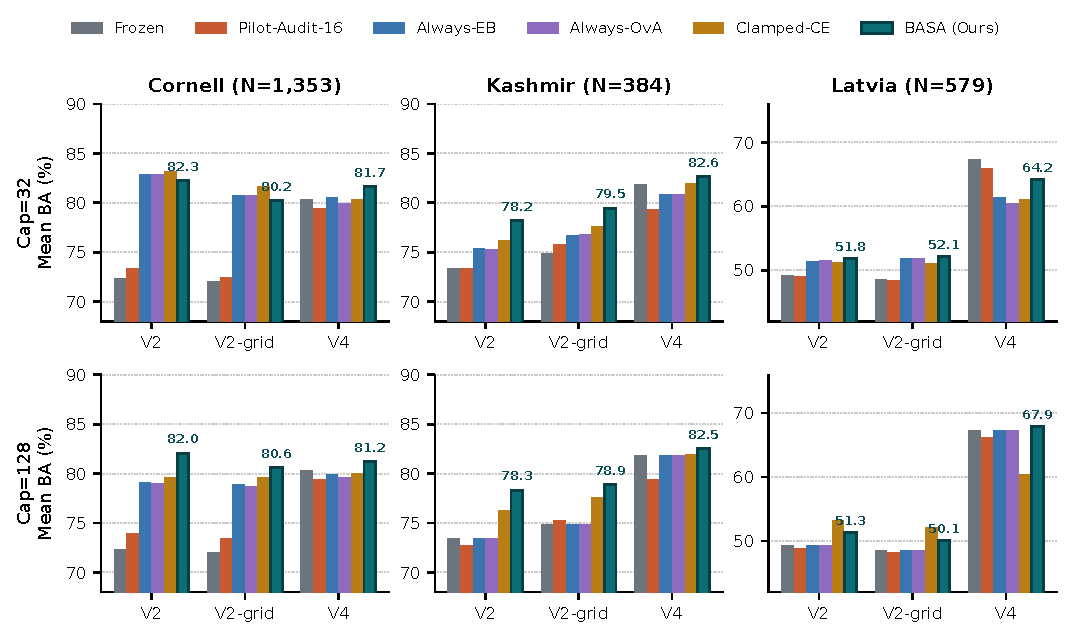
\includegraphics[width=\textwidth]{figures/compag_main_comparison.pdf}
  \caption{Per-site and per-backbone mean balanced accuracy under zero-initial-credit (\emph{earned}) funding at the 25\% uplink rate (1,700~B/frame) for 32-label (top) and 128-label (bottom) authorization caps. Including budget-clamped \emph{Clamped-CE} removes overflow crashes on Kashmir/Latvia (\texttt{Cap=128}), yet BASA still wins 14/18 earned settings by combining tighter earned amortization with source-anchored regularization.}
  \label{fig:main}
\end{figure}

\begin{table}[t]
\centering
\caption{Detailed mean balanced accuracy (\%) across all 36 primary settings at the 25\% uplink rate (1,700~B/frame). \emph{Clmp-CE} denotes budget-clamped cross-entropy ($k \le k_{\mathrm{half}}$).}
\label{tab:full36}
\scriptsize
\setlength{\tabcolsep}{2.8pt}
\resizebox{\textwidth}{!}{%
\begin{tabular}{@{}ll|rrrrrr|rrrrrr@{}}
\toprule
& & \multicolumn{6}{c|}{Prepaid byte grant (upfront)} & \multicolumn{6}{c}{Earned byte grant (zero initial credit)} \\
\cmidrule(lr){3-8}\cmidrule(lr){9-14}
Site & Pipe. & Frozen & Pilot16 & EB-rk & OvA & Clmp-CE & \textbf{BASA} & Frozen & Pilot16 & EB-rk & OvA & Clmp-CE & \textbf{BASA} \\
\midrule
\multicolumn{14}{@{}l}{\emph{Panel A: 32-label authorization cap}} \\
Cornell & V2      & 72.35 & 73.20 & 84.06 & 84.34 & \textbf{84.68} & 83.46 & 72.35 & 73.32 & 82.84 & 82.89 & \textbf{83.22} & 82.26 \\
        & V2-grid & 72.03 & 72.39 & 81.31 & 81.61 & \textbf{82.41} & 80.80 & 72.05 & 72.49 & 80.70 & 80.73 & \textbf{81.61} & 80.22 \\
        & V4      & 80.43 & 79.73 & 81.16 & 80.52 & 81.00 & \textbf{82.57} & 80.33 & 79.40 & 80.54 & 79.90 & 80.32 & \textbf{81.66} \\
Kashmir & V2      & 73.32 & 73.15 & 83.99 & 83.57 & \textbf{84.21} & 83.25 & 73.40 & 73.39 & 75.40 & 75.29 & 76.23 & \textbf{78.18} \\
        & V2-grid & 75.20 & 76.25 & 83.79 & 83.86 & \textbf{83.94} & 83.72 & 74.84 & 75.78 & 76.71 & 76.75 & 77.57 & \textbf{79.45} \\
        & V4      & 82.54 & 81.25 & 89.12 & 88.62 & \textbf{89.70} & 85.95 & 81.84 & 79.35 & 80.84 & 80.83 & 81.95 & \textbf{82.64} \\
Latvia  & V2      & 48.76 & 48.23 & 50.28 & \textbf{50.83} & 50.12 & 50.52 & 49.26 & 49.01 & 51.32 & 51.51 & 51.16 & \textbf{51.85} \\
        & V2-grid & 49.06 & 49.31 & 51.94 & \textbf{52.82} & 51.60 & 50.94 & 48.57 & 48.44 & 51.79 & 51.84 & 51.06 & \textbf{52.14} \\
        & V4      & \textbf{67.12} & 64.95 & 57.88 & 57.10 & 57.47 & 63.22 & \textbf{67.32} & 65.90 & 61.34 & 60.45 & 61.02 & 64.16 \\
\midrule
\multicolumn{14}{@{}l}{\emph{Panel B: 128-label authorization cap}} \\
Cornell & V2      & 72.35 & 73.20 & 85.31 & 85.51 & \textbf{86.68} & 86.64 & 72.35 & 73.98 & 79.10 & 79.01 & 79.62 & \textbf{82.05} \\
        & V2-grid & 72.03 & 72.98 & 82.66 & 83.16 & \textbf{84.78} & 84.29 & 72.05 & 73.43 & 78.94 & 78.66 & 79.65 & \textbf{80.58} \\
        & V4      & 80.43 & 79.87 & 84.04 & 83.62 & \textbf{84.25} & 84.14 & 80.33 & 79.36 & 79.88 & 79.58 & 79.98 & \textbf{81.23} \\
Kashmir & V2      & 73.32 & 73.15 & 73.32 & 73.32 & \textbf{84.19} & 81.75 & 73.40 & 72.73 & 73.40 & 73.40 & 76.21 & \textbf{78.32} \\
        & V2-grid & 75.20 & 74.67 & 75.20 & 75.20 & \textbf{83.88} & 82.24 & 74.84 & 75.24 & 74.84 & 74.84 & 77.57 & \textbf{78.88} \\
        & V4      & 82.54 & 80.93 & 82.54 & 82.54 & \textbf{89.76} & 87.81 & 81.84 & 79.35 & 81.84 & 81.84 & 81.94 & \textbf{82.51} \\
Latvia  & V2      & 48.76 & 48.23 & 48.76 & 48.76 & 49.99 & \textbf{51.10} & 49.26 & 48.87 & 49.26 & 49.26 & \textbf{53.18} & 51.27 \\
        & V2-grid & 49.06 & 49.31 & 49.06 & 49.06 & 51.43 & \textbf{53.08} & 48.57 & 48.22 & 48.57 & 48.57 & \textbf{52.18} & 50.10 \\
        & V4      & \textbf{67.12} & 64.95 & \textbf{67.12} & \textbf{67.12} & 60.20 & 65.26 & 67.32 & 66.14 & 67.32 & 67.32 & 60.38 & \textbf{67.92} \\
\bottomrule
\end{tabular}}
\end{table}

\subsection{Component Ablation, Tail-Risk Stability, and Uplink Bandwidth Sweep}
\label{sec:ablation}

Fig.~\ref{fig:ablation}(a) and the per-seed distribution across all 720 runs at the 25\% rate clarify the distinct roles of BASA's three components:
\begin{itemize}
  \item \textbf{Horizon Amortization} is the main driver of mean balanced accuracy: removing it (\emph{w/o Amortization}) drops overall mean $\BA$ from \textbf{73.50\% to 71.99\%} ($-1.51$~pp), hitting short-horizon Kashmir ($-2.91$~pp) and V2/V2-grid ($-2.10$/$-1.97$~pp) hardest.
  \item \textbf{ASAR Source Anchoring} acts as a backbone-aware safeguard: without being told which model is deployed, OOF selection chooses unanchored fitting ($\lambda = 1$) in \textbf{79.8\%} of V2 runs and \textbf{74.8\%} of V2-grid runs, yet automatically switches to source anchoring ($\lambda \in \{5, 25, \infty\}$) in \textbf{86.8\%} of MobileNetV4 runs. Fixing $\lambda = 1$ (\emph{w/o ASAR}) nudges V2/V2-grid up by 0.3--0.6~pp, but costs \textbf{$-1.30$~pp} on MobileNetV4 (77.42\% $\to$ 76.12\%) and \textbf{$-1.12$~pp} on Latvia (55.96\% $\to$ 54.84\%).
  \item \textbf{Quantile Stratification} trades a tiny mean difference for lower tail risk on skewed reservoirs: removing it (\emph{w/o Stratified Sel.}) gives 73.63\% overall (+0.13~pp) because random sampling slightly favors Kashmir's relatively balanced pool (+0.71~pp). On the imbalanced orchards, however, stratification raises both mean and worst-draw performance: worst-draw $\BA$ improves by \textbf{+0.65~pp} on Cornell (79.03\% vs.\ 78.38\%) and \textbf{+1.28~pp} on Latvia (45.97\% vs.\ 44.69\%), lifting the global worst run from 40.21\% to 41.13\% while lowering cross-seed standard deviation (3.01\% vs.\ 3.09\%).
\end{itemize}

Fig.~\ref{fig:ablation}(b) traces performance from scarce \textbf{10\% (680~B/frame)} to abundant \textbf{50\% (3,400~B/frame)} uplinks. BASA's advantage is sharpest where bandwidth is tightest: at \textbf{10\%}, BASA reaches \textbf{70.49\%}, outperforming \emph{Always-CE} (+2.65~pp), \emph{Frozen} (+2.77~pp), and \emph{Clamped-CE} (69.40\%, \textbf{+1.09~pp}). At \textbf{25\%}, BASA remains first (73.50\% vs.\ 72.92\% \emph{Clamped-CE}). At a generous \textbf{50\%} uplink, however, \emph{Clamped-CE} (75.56\%) and \emph{Clamped-EB-rank} (75.36\%) edge slightly ahead of BASA (75.29\%, $-0.27$~pp), because abundant bandwidth removes the setup-starvation penalty and rewards buying up to $0.5B$ labels.

\begin{figure}[t]
  \centering
  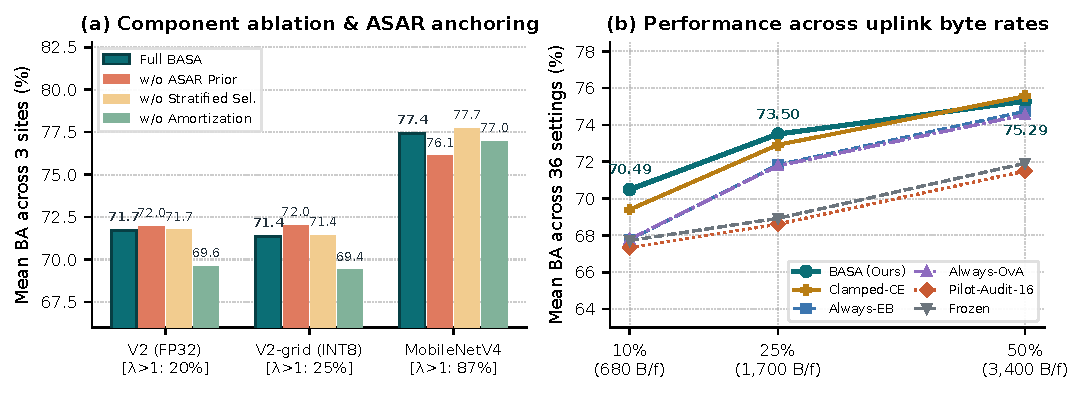
\includegraphics[width=\textwidth]{figures/compag_ablation_and_sweep.pdf}
  \caption{(a) Component ablation per backbone at the 25\% byte rate, annotated with ASAR's automatic source-anchoring rate ($\lambda > 1$: 20\% V2, 25\% V2-grid, 87\% MobileNetV4). (b) Mean balanced accuracy across all 36 settings from 10\% to 50\% uplink rates, showing BASA's lead under scarce uplinks (10\% and 25\%) and the 50\% crossover with budget-clamped \emph{Clamped-CE}.}
  \label{fig:ablation}
\end{figure}

\subsection{MCU Quantization Sensitivity and Router Rank Reversals}
\label{sec:quant}

To isolate numerical precision from label-budgeting effects, we replayed the 128-label Cornell-trained online deferral benchmark across all 10 distinct routing policies (45 method pairs) when moving head fitting and serving between FP32 and the ESP32-S3 INT8 quantization grid, transferring the Cornell-fitted routers to both the Cornell evaluation split (1,353 images) and the complete 1,190-image Latvian archive (Fig.~\ref{fig:ranks}). Serving FP32-fitted heads on quantized activations reverses \textbf{6/45} pairwise rankings on Cornell (where OvA overtakes Continued CE, 80.24\% vs.\ 79.88\%) and \textbf{13/45} rankings on Latvia. Refitting directly on quantized grid activations eliminates reversals on Cornell (0/45, restoring Continued CE at 83.70\%) but leaves \textbf{10/45} reversals on Latvia. Small FP32 gains reported for deferral routers therefore cannot be assumed to survive INT8 microcontroller deployment unless heads are both fitted and validated on quantized activations.

\begin{figure}[t]
  \centering
  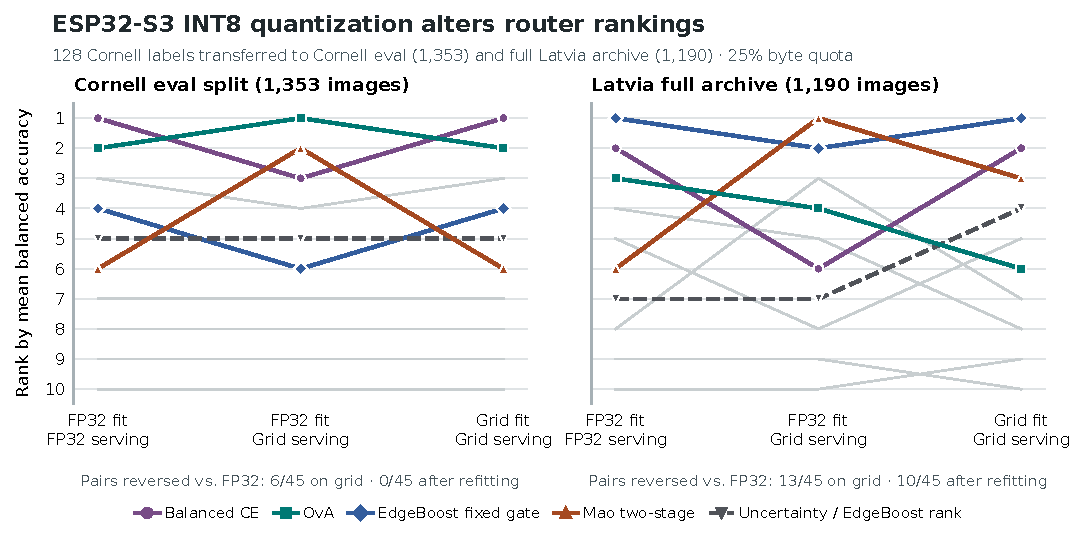
\includegraphics[width=\textwidth]{figures/compag_precision_ranks.pdf}
  \caption{Effect of ESP32-S3 host INT8 quantization on the relative ordering of 10 online deferral policies trained on 128 Cornell labels and evaluated at a 25\% byte quota on the Cornell evaluation split (1,353 images) and the full Latvian archive (1,190 images).}
  \label{fig:ranks}
\end{figure}

\subsection{Latvian Apple-Scab Diagnostics and One-Sided Recall Guard}
\label{sec:latvia}

On the nine chronological Latvian evaluation dates (507 scab positives, 72 negatives), native local discrimination diverges sharply across backbones: V2 achieves only 0.449 source AUROC (0.408 on V2-grid; oracle threshold ceiling 51.57\% $\BA$), whereas MobileNetV4 reaches 0.791 source AUROC (oracle ceiling 74.07\% $\BA$). Because Latvia's negative label means ``no visible apple scab'' rather than strictly healthy foliage, factory models trained for general disease suffer severe operating-point mismatch: V2 starts with 67 false alarms and 49 misses, while V4 starts with 12 false alarms and 227 misses.

Table~\ref{tab:guard} evaluates the one-sided recall guard under earned credit (\texttt{Cap=32}, 25\% rate). Without buying any labels, \emph{Frozen+Guard} cuts V2 misses from 49.0 to 31.0 and V2-grid misses from 68.0 to 45.0 with zero added false alarms. Pairing BASA with the recall guard (\emph{BASA+Guard}) lowers misses further to \textbf{23.9} on V2 ($-51.2\%$) and \textbf{28.1} on V2-grid ($-58.7\%$) while raising $\BA$ to 50.66\% and 50.11\%. On MobileNetV4, \emph{BASA+Guard} cuts misses from 227.0 to \textbf{153.8} ($-32.2\%$) at the cost of 13.4 additional false alarms (25.4 vs.\ 12.0), underscoring that threshold-guarding choices depend on the relative agronomic cost of missed outbreaks versus extra manual checks.

\begin{table}[t]
\centering
\caption{Latvia chronological holdout (507 positives, 72 negatives): false alarms / misses / $\BA$ (\%) under 25\% earned credit (\texttt{Cap=32}).}
\label{tab:guard}
\small
\begin{tabular}{@{}lccc@{}}
\toprule
Policy & V2 (FP / FN / $\BA$) & V2-grid (FP / FN / $\BA$) & V4 (FP / FN / $\BA$) \\
\midrule
Native (0~B)            & 67.0 / 49.0 / 48.64 & 67.0 / 68.0 / 46.77 & 12.0 / 227.0 / 69.28 \\
Frozen + Guard          & 67.0 / 31.0 / 50.42 & 67.0 / 45.0 / 49.03 & 12.0 / 206.0 / \textbf{71.35} \\
Pilot-Audit-16 + Guard  & 67.0 / 32.0 / 50.32 & 67.0 / 47.0 / 48.84 & 15.1 / 196.1 / 70.21 \\
\textbf{BASA + Guard}   & 67.7 / \textbf{23.9} / \textbf{50.66} & 67.8 / \textbf{28.1} / \textbf{50.11} & 25.4 / \textbf{153.8} / 67.19 \\
\bottomrule
\end{tabular}
\end{table}

\subsection{On-Chip ESP32-S3 Silicon Validation and Rural Link Deadlines}
\label{sec:hardware}

Table~\ref{tab:hw} summarizes direct hardware measurements obtained by flashing our standalone C99 benchmark (\texttt{esp32s3\_bench}, compiled with \texttt{xtensa-esp32s3-elf-gcc 14.2.0}, ESP-IDF v5.4.4) onto a physical ESP32-S3 N16R8 board (QFN56 rev~v0.2, dual-core Xtensa LX7 at 160~MHz, 16~MB Flash, 8~MB Octal PSRAM at 80~MHz), matching the clock speed and toolchain of the published AgriTinyVision v0.2 backbone benchmark \citep{agri}.

Across 1,000 steady-state runs timed with \texttt{esp\_timer\_get\_time()}, BASA's on-chip compute cost is negligible beside the 527.84~ms MobileNetV2-160 INT8 backbone:
\begin{itemize}
  \item \textbf{\texttt{EQ01} head inference} (1,280-D INT8 dot product, L2 norm, and bias): \textbf{93~$\mu$s} median (93~$\mu$s P95, 99~$\mu$s P99)---0.018\% of backbone latency.
  \item \textbf{Causal 64-frame rolling gate:} \textbf{41~$\mu$s} median (45~$\mu$s P95/P99), giving \textbf{134~$\mu$s (0.134~ms, 0.025\% of backbone time)} combined per-frame overhead.
  \item \textbf{OTA parse and calibration quantization:} parsing the 1,294-B \texttt{EQ01} packet takes \textbf{50~$\mu$s} once per update; quantizing a 1,280-D FP32 activation vector to signed INT8 takes \textbf{565~$\mu$s} median (573~$\mu$s P95/P99), incurred only on the $k$ calibration frames.
  \item \textbf{Bit-exact parity and memory:} on-chip execution matches Python with \textbf{0/16 mismatches} ($0.0$ max absolute error, complementing 0/81,180 host C99 parity), using \textbf{1,836~B} of persistent state (0.64\% of AgriTinyVision's 286~KB free SRAM) and \textbf{0~B} of PSRAM (8,386,188~B unchanged).
\end{itemize}

Replaying link deadlines over nine Norwegian forestry private-5G traces (8--179~Mbit/s uplink, 12--27~ms RTT; \citealp{forest}) shows every remote query returns well within 2~s. Under a harsh synthetic narrowband link (10/20~kbit/s, 1.2~s RTT, 10\% packet loss, 60~s periodic outages), zero replies meet a 2~s deadline (falling back cleanly to local BASA calls), while a 30~s scouting deadline recovers 85.0 of 166.4 remote replies on Cornell (82.36\% vs.\ 84.76\% with instantaneous replies).

\begin{table}[t]
\centering
\caption{Direct on-chip ESP32-S3 N16R8 silicon benchmark (160~MHz, ESP-IDF v5.4.4, 1,000 runs) and AgriTinyVision v0.2 hardware anchor.}
\label{tab:hw}
\small
\resizebox{\textwidth}{!}{%
\begin{tabular}{@{}lr@{}}
\toprule
Metric / Component & Measured hardware value \\
\midrule
Target silicon & ESP32-S3 N16R8 (160~MHz, 16~MB Flash, 8~MB PSRAM) \\
Backbone INT8 latency (P50 / P95) \citep{agri} & 527.84~ms / 527.85~ms \\
AgriTinyVision free SRAM / PSRAM \citep{agri} & 286,447~B / 5,046,852~B \\
\midrule
BASA wire head packet (\texttt{EQ01}) & 1,294~B (over-the-air update) \\
BASA persistent state (\texttt{head} + \texttt{gate}) & 1,292~B + 544~B = 1,836~B (0.64\% SRAM) \\
On-chip PSRAM delta (before / after) & 0~B (8,386,188~B unchanged) \\
\textbf{On-chip \texttt{EQ01} parse (P50 / P95 / P99)} & \textbf{50 / 50 / 50~$\mu$s} \\
\textbf{On-chip \texttt{EQ01} inference (P50 / P95 / P99)} & \textbf{93 / 93 / 99~$\mu$s} (0.018\% backbone) \\
\textbf{On-chip streaming gate (P50 / P95 / P99)} & \textbf{41 / 45 / 45~$\mu$s} \\
\textbf{On-chip FP32$\to$INT8 quant.\ (P50 / P95 / P99)} & \textbf{565 / 573 / 573~$\mu$s} (cal.\ frames only) \\
On-chip ESP32-S3 bit-exact parity & 0 / 16 mismatches ($0.0$ max abs.\ err.) \\
Host C99 full-cohort parity & 0 / 81,180 mismatches ($<10^{-12}$ max err.) \\
\bottomrule
\end{tabular}}
\end{table}

\section{Discussion}
\label{sec:discussion}

\subsection{Practical Implications for Orchard Deployment}
The paired results point to three concrete engineering choices when deploying bandwidth-limited cameras in orchards. First, supervision budgets should match the link's funding schedule: when credit accrues incrementally without borrowing, capping paid calibration near 25\% of window bytes prevents long unadapted startup delays, whereas abundant uplinks ($\ge 50\%$) allow larger label batches up to $0.5B$ without starving deferral. Second, small-sample adaptation on modern backbones such as MobileNetV4 should never discard the factory classifier direction; ASAR preserves pretrained ordering automatically when $k$ is small while relaxing toward full linear adaptation on weaker source heads like MobileNetV2. Third, router selection should be verified on quantized activations rather than FP32, and the one-sided recall guard should be enabled whenever missed foliar outbreaks are substantially costlier than extra field checks.

\subsection{Limitations}
Three scope limits should be kept in mind. First, although BASA's \texttt{EQ01} head, quantization kernel, and streaming gate ran directly on ESP32-S3 N16R8 silicon (Table~\ref{tab:hw}) and match 59/60 archived board logs, the 3,000+ cross-site V2-grid activations rely on host ESP-PPQ replay (fixture codes $(56,-62)$ vs.\ $(58,-59)$ on silicon), and board-level battery draw during live cellular or LoRa transmission remains for future field trials. Second, Latvia's single-pathogen scab reference mixes label-definition shift with visual domain shift, and real human annotation turnaround (32--128~min at 15--60~s per photograph) introduces wall-clock latency beyond instantaneous byte replays. Third, leaf-level screening photographs serve as field scouting triggers rather than whole-tree agronomic diagnoses.

\section{Conclusion}
\label{sec:conclusion}

We formulated paid remote annotation and strictly causal single-frame deferral for bandwidth-limited orchard cameras on a unified byte ledger under both prepaid and zero-initial-credit (earned) schedules, and proposed BASA. By pairing horizon-amortized supervision budgeting, label-free quantile-stratified selection, and convex anisotropic source-anchored regularization (ASAR) packed into a 1,294-byte \texttt{EQ01} INT8 head, BASA achieves the highest mean balanced accuracy across all 36 primary 25\%-uplink settings (73.50\% overall, 72.52\% earned) and at a 10\% scarce uplink (70.49\%), outperforming both fixed-cap and budget-clamped published deferral baselines while documenting the 50\% abundant-uplink crossover. Direct benchmarking on ESP32-S3 N16R8 silicon confirms 134~$\mu$s combined per-frame overhead (0.025\% of backbone inference), 1,836~B persistent RAM, and zero bit-level mismatches.

\section*{CRediT authorship contribution statement}
\textbf{Weicheng Tong:} Conceptualization, Methodology, Software, Validation, Formal analysis, Investigation, Data curation, Writing -- original draft, Writing -- review \& editing, Visualization.

\section*{Declaration of competing interest}
The author declares that he has no known competing financial interests or personal relationships that could have appeared to influence the work reported in this paper.

\section*{Data availability}
All underlying apple-leaf datasets and rural 5G traces are publicly available from their original providers \citep{singh2020,cornell,kashmir,latvia,forest}. Source code, C99 reference implementations, ESP32-S3 benchmark firmware, and aggregated verification tables are maintained in the unified AgriTinyVision repository (\url{https://github.com/Sver0411/AgriTinyVision}, under \texttt{research/field-edge-audit}).

\section*{Declaration of generative AI and AI-assisted technologies in the writing process}
During the preparation of this work, the author used generative AI tools to assist with language editing, experiment-script drafting, and \LaTeX{} formatting. After using these tools, the author reviewed, verified, and edited all code, C99 and ESP32-S3 hardware measurements, statistical analyses, and manuscript text, and takes full responsibility for the content of the publication.

\bibliographystyle{elsarticle-harv}
\bibliography{references}

\end{document}
